\documentclass[11pt]{article}
\usepackage[a4paper,margin=1in]{geometry}
\usepackage{amsmath,amssymb,amsthm,mathtools}
\usepackage{booktabs}
\usepackage{enumitem}
\usepackage{graphicx}
\usepackage{microtype}
\usepackage{hyperref}
\usepackage[nameinlink,capitalise]{cleveref}
\usepackage[numbers,sort&compress]{natbib}

\newtheorem{theorem}{Theorem}[section]
\newtheorem{proposition}[theorem]{Proposition}
\newtheorem{corollary}[theorem]{Corollary}
\newtheorem{lemma}[theorem]{Lemma}
\theoremstyle{definition}
\newtheorem{definition}[theorem]{Definition}
\theoremstyle{remark}
\newtheorem{remark}[theorem]{Remark}
\newcommand{\norm}[1]{\left\lVert#1\right\rVert}
\newcommand{\tr}{\operatorname{tr}}
\newcommand{\PhiR}{\Phi_r}

\title{Gap-Weighted Weak-Mode Quotients\\
\large Adaptive Ritz Enrichment Without Unstable Direction Recovery}
\author{Liang Wang}
\date{July 2026}

\begin{document}
\maketitle

\begin{abstract}
RH-95 showed that the fourth projected-cross direction can be almost null:
its singular value may be eleven orders of magnitude below the leading mode.
Geometric reconstruction is then unstable, even though the corrected Ritz
tail is insensitive to the direction.  We replace weak-direction
identification by an energy quotient.

For a positive block compression
\[
 H=\begin{pmatrix}A&C\\C^*&D\end{pmatrix},
\]
let $\Phi_r(H)$ denote the sum of its largest $r$ eigenvalues.  We first prove
the universal omitted-block bound
\[
 0\le\Phi_r(H)-\Phi_r(A)
 \le 2\norm C_*+\tr D.
\]
More sharply, suppose the retained rank-$r$ cutoff satisfies
$\lambda_r^\downarrow(A)\ge\alpha$, while $D\le\beta I$ with
$\alpha>\beta$.  Our gap-weighted weak-mode tail-loss theorem gives
\[
 0\le\Phi_r(H)-\Phi_r(A)
 \le\frac{\norm C_F^2}{\alpha-\beta}.
\]
The proof optimizes the amount of a rank-$r$ projector entering the omitted
block and requires no identification of its weak basis vectors.

We audit adaptive projected-cross widths at relative singular cutoffs
$10^{-8},10^{-6},10^{-4}$ over the 120 source-seeded updates.  At the primary
cutoff $10^{-8}$, exactly five weak fourth modes are omitted.  All five losses
are gap-certified, all updates remain Ritz-monotone, and all ten endpoints
stay below the $1.01$ target; the worst endpoint/reference ratio is
$1.001173$.  The largest adaptive/full one-step tail ratio is $1.00000465$.
More aggressive cutoffs reveal the next obstruction.  Every local omission
is still certified, but the recursive endpoint target fails: the worst ratios
are $1.024922$ at $10^{-6}$ and $1.014092$ at $10^{-4}$.

Thus the ill-conditioned fourth mode can be quotiented safely at the five
identified updates, but local certificates do not compose automatically.
The next task is a horizon recurrence for accumulated quotient losses.  No
uniform gap theorem, Hilbert--Polya operator, zero identification, or Riemann
Hypothesis result is claimed.
\end{abstract}

\noindent\textbf{Keywords:} Ky Fan sum; Ritz enrichment; weak singular mode;
spectral gap; adaptive rank; validated numerics.

\medskip
\noindent\textbf{MSC 2020:} 47A75; 15A18; 65F15; 65G20; 37C30.

\section{Introduction}

The source-seeded chain of RH-94 uses four projected-cross directions to
track the ambient leading packet over a complete finite prefix
\citep{WangSourceSeed2026}.  RH-95 reduced the ambient cross SVD to
packet-scale normal matrices, but found that the fourth cross mode can be
extremely ill conditioned \citep{WangCrossMoment2026}.  In the weakest
updates, different stabilized fourth directions produce visibly different
projectors but nearly identical corrected tails.

This suggests that geometric identification is stronger than the route
needs.  The packet is used to control captured energy and subsequent tail
propagation.  If adjoining a weak direction can improve the leading rank-$r$
capture by at most a certified tolerance, then that direction should be
quotiented rather than reconstructed.

The basic finite-dimensional problem is as follows.  A retained enrichment
produces a positive matrix $A$.  Additional weak directions enlarge it to
\[
 H=\begin{pmatrix}A&C\\C^*&D\end{pmatrix}.
\]
How much can the leading rank-$r$ Ky Fan sum increase?  A universal answer
comes from trace-norm perturbation.  A sharper answer uses two pieces of
structure: the $r$th retained Ritz value lies above the omitted diagonal
spectrum, and the coupling $C$ is small.

The resulting gap-weighted estimate is elementary but useful.  It bounds the
energy value of the entire omitted subspace without selecting a stable basis
inside that subspace.  It therefore matches the exact obstruction exposed by
RH-95.

The audit then asks a second question: how aggressively can weak modes be
removed along the recursive source-to-endpoint chain?  A cutoff at $10^{-8}$
removes exactly the five directions already identified as unstable and
preserves every endpoint.  Larger cutoffs fail, even though each individual
loss remains locally certified.  This separates local quotient validity from
global horizon composition.

\section{Ky Fan formulation}
\label{sec:kyfan}

For a Hermitian matrix $X$, define
\[
 \Phi_r(X)=\sum_{j=1}^r\lambda_j^\downarrow(X)
 =\max_{\substack{P=P^*=P^2\\\tr P=r}}\tr(PX).
\]
The variational equality is Ky Fan's maximum principle
\citep{Fan1949,Bhatia1997}.

Let
\begin{equation}
 H=\begin{pmatrix}A&C\\C^*&D\end{pmatrix}\ge0,
 \qquad A\in\mathbb C^{m\times m},\quad m\ge r.
 \label{eq:block}
\end{equation}
The retained Ritz construction uses $\Phi_r(A)$, whereas adding the weak
directions makes $\Phi_r(H)$ available.  Their difference is exactly the
captured-energy loss caused by quotienting the omitted block.

\begin{theorem}[Universal omitted-block bound]
\label{thm:universal}
For \eqref{eq:block},
\begin{equation}
 0\le\Phi_r(H)-\Phi_r(A)
 \le 2\norm C_*+\tr D.
 \label{eq:universal}
\end{equation}
\end{theorem}

\begin{proof}
Embed $A$ as $H_0=\operatorname{diag}(A,0)$.  Since $A\ge0$ and $m\ge r$,
$\Phi_r(H_0)=\Phi_r(A)$.  Enlargement of the trial space gives the lower
bound.  The Ky Fan sum is Lipschitz in trace norm:
\[
 |\Phi_r(H)-\Phi_r(H_0)|\le\norm{H-H_0}_*.
\]
Now
\[
 H-H_0=
 \begin{pmatrix}0&C\\C^*&0\end{pmatrix}
 +\begin{pmatrix}0&0\\0&D\end{pmatrix}.
\]
The first matrix has trace norm $2\norm C_*$, and the second has trace norm
$\tr D$ because $D\ge0$.
\end{proof}

The universal bound needs no gap, but it counts all omitted diagonal energy.
For a weak direction whose diagonal energy is not itself small, it can be too
large for a relative tail budget.

\section{Gap-weighted weak-mode tail-loss theorem}
\label{sec:gap}

\begin{theorem}[Gap-weighted weak-mode tail-loss theorem]
\label{thm:gap}
Assume in \eqref{eq:block} that
\[
 \lambda_r^\downarrow(A)\ge\alpha,\qquad D\le\beta I,
 \qquad \delta:=\alpha-\beta>0.
\]
Then
\begin{equation}
 0\le\Phi_r(H)-\Phi_r(A)
 \le\frac{\norm C_F^2}{\delta}.
 \label{eq:gap-bound}
\end{equation}
\end{theorem}

\begin{proof}
Let $P$ be any rank-$r$ orthogonal projector on the full block space and
write
\[
 P=\begin{pmatrix}P_{11}&P_{12}\\P_{12}^*&P_{22}\end{pmatrix},
 \qquad t=\tr P_{22}.
\]
Since $0\le P_{11}\le I$ and $\tr P_{11}=r-t$, the variational description of
partial spectral mass gives
\begin{equation}
 \tr(P_{11}A)\le\Phi_r(A)-\alpha t.
 \label{eq:a-mass}
\end{equation}
Also $\tr(P_{22}D)\le\beta t$.  From $P^2=P$,
\[
 P_{12}^*P_{12}=P_{22}-P_{22}^2,
\]
so $\norm{P_{12}}_F^2\le t$.  Therefore
\begin{align*}
 \tr(PH)-\Phi_r(A)
 &\le-\delta t+2\operatorname{Re}\tr(P_{12}C^*)\\
 &\le-\delta t+2\norm C_F\sqrt t\\
 &\le\frac{\norm C_F^2}{\delta}.
\end{align*}
The last line maximizes the scalar quadratic in $\sqrt t$.  Taking the maximum
over rank-$r$ projectors $P$ proves the upper bound.  The lower bound again
follows by retaining the old trial space.
\end{proof}

\begin{remark}
The theorem identifies the correct quotient data.  It does not require the
omitted cross singular value itself, nor a stable orientation of its left
singular vector.  It requires only a coupling norm and a retained-to-omitted
compressed spectral gap.
\end{remark}

\subsection{Adaptive width}

Let
\[
 s_1(K)\ge s_2(K)\ge\cdots
\]
be projected-cross singular values.  Given a relative threshold $\tau$ and
width limits $k_{\min}\le k_{\max}$, define
\begin{equation}
 k_\tau
 =\max\left\{k_{\min},
 \min\left(k_{\max},
 \#\{j\le k_{\max}:s_j(K)/s_1(K)\ge\tau\}\right)\right\}.
 \label{eq:adaptive}
\end{equation}
The retained enrichment uses the first $k_\tau$ directions.  The remaining
directions up to $k_{\max}$ form the omitted block in
\cref{thm:gap}.

The rule is deliberately local.  It says which directions are weak at one
update.  It does not yet allocate a global horizon error budget.

\section{Validated audit}
\label{sec:audit}

\subsection{Protocol}

We replay the five scales and two directional channels of RH-94, from the
source seed to endpoints $4,6,11,17,22$.  The rank clock is unchanged, with
minimum and maximum enrichment widths two and four.  Three relative cutoffs
are tested:
\[
 \tau\in\{10^{-8},10^{-6},10^{-4}\}.
\]
Each threshold runs its own recursive chain, so endpoint behavior need not be
monotone in $\tau$.

At every omitted update, the retained and full-width bases are assembled in
one ordered QR factorization.  The compressed blocks $A,C,D$ are then
extracted from the same full matrix.  Binary64 eigendecompositions are
inflated by their reconstruction residuals and a roundoff guard to obtain a
lower bound for $\alpha$ and an upper bound for $\beta$.  Tail forms are
evaluated from exact binary inputs in Arb at 384-bit precision
\citep{Rump2010}.

\subsection{Primary cutoff}

At $\tau=10^{-8}$, the adaptive chain omits the fourth direction in exactly
five of 120 updates.  These are the five weak-mode events identified by the
conditioning audit of RH-95.  Every omitted update has a positive certified
gap and satisfies \eqref{eq:gap-bound}.

The chain uses width three five times and width four 115 times.  All direct
Ritz steps are monotone.  The largest adaptive/full-width one-step tail ratio
is
\[
 1.0000046481.
\]
All ten endpoint/reference ratios remain below $1.01$, with maximum
\[
 1.0011723197.
\]
Thus unstable fourth-mode inversion is unnecessary at precisely the updates
where it is least meaningful.

The gap bounds are conservative.  The largest primary bound is about
$5085$ times its observed one-step loss, but remains below
$2.90\times10^{-4}$ of the corresponding full-width tail.  This is adequate
for the finite local decision.

\subsection{Aggressive cutoffs and the composition barrier}

\begin{table}[t]
\centering
\caption{Adaptive threshold summary over 120 updates.}
\label{tab:thresholds}
\begin{tabular}{@{}lrrrrr@{}}
\toprule
$\tau$ & width 2 & width 3 & width 4 & omitted & worst endpoint\\
\midrule
$10^{-8}$ & 0 & 5 & 115 & 5  & 1.001173\\
$10^{-6}$ & 1 & 10 & 109 & 11 & 1.024922\\
$10^{-4}$ & 5 & 17 & 98  & 22 & 1.014092\\
\bottomrule
\end{tabular}
\end{table}

The two larger thresholds fail the endpoint gate, as shown in
\cref{tab:thresholds}.  This does not come from an invalid local theorem:
all eleven omissions at $10^{-6}$ and all twenty-two omissions at $10^{-4}$
have green gap certificates.  Instead, small one-step losses alter the packet
fed into later updates and accumulate nonlinearly.

The recursive response is not monotone in the threshold.  The $10^{-6}$ chain
has a worse endpoint than the $10^{-4}$ chain even though it omits fewer
directions.  Once the packet paths diverge, a larger local trial space at one
time does not imply a nested trial space at all later times.

\begin{figure}[t]
\centering
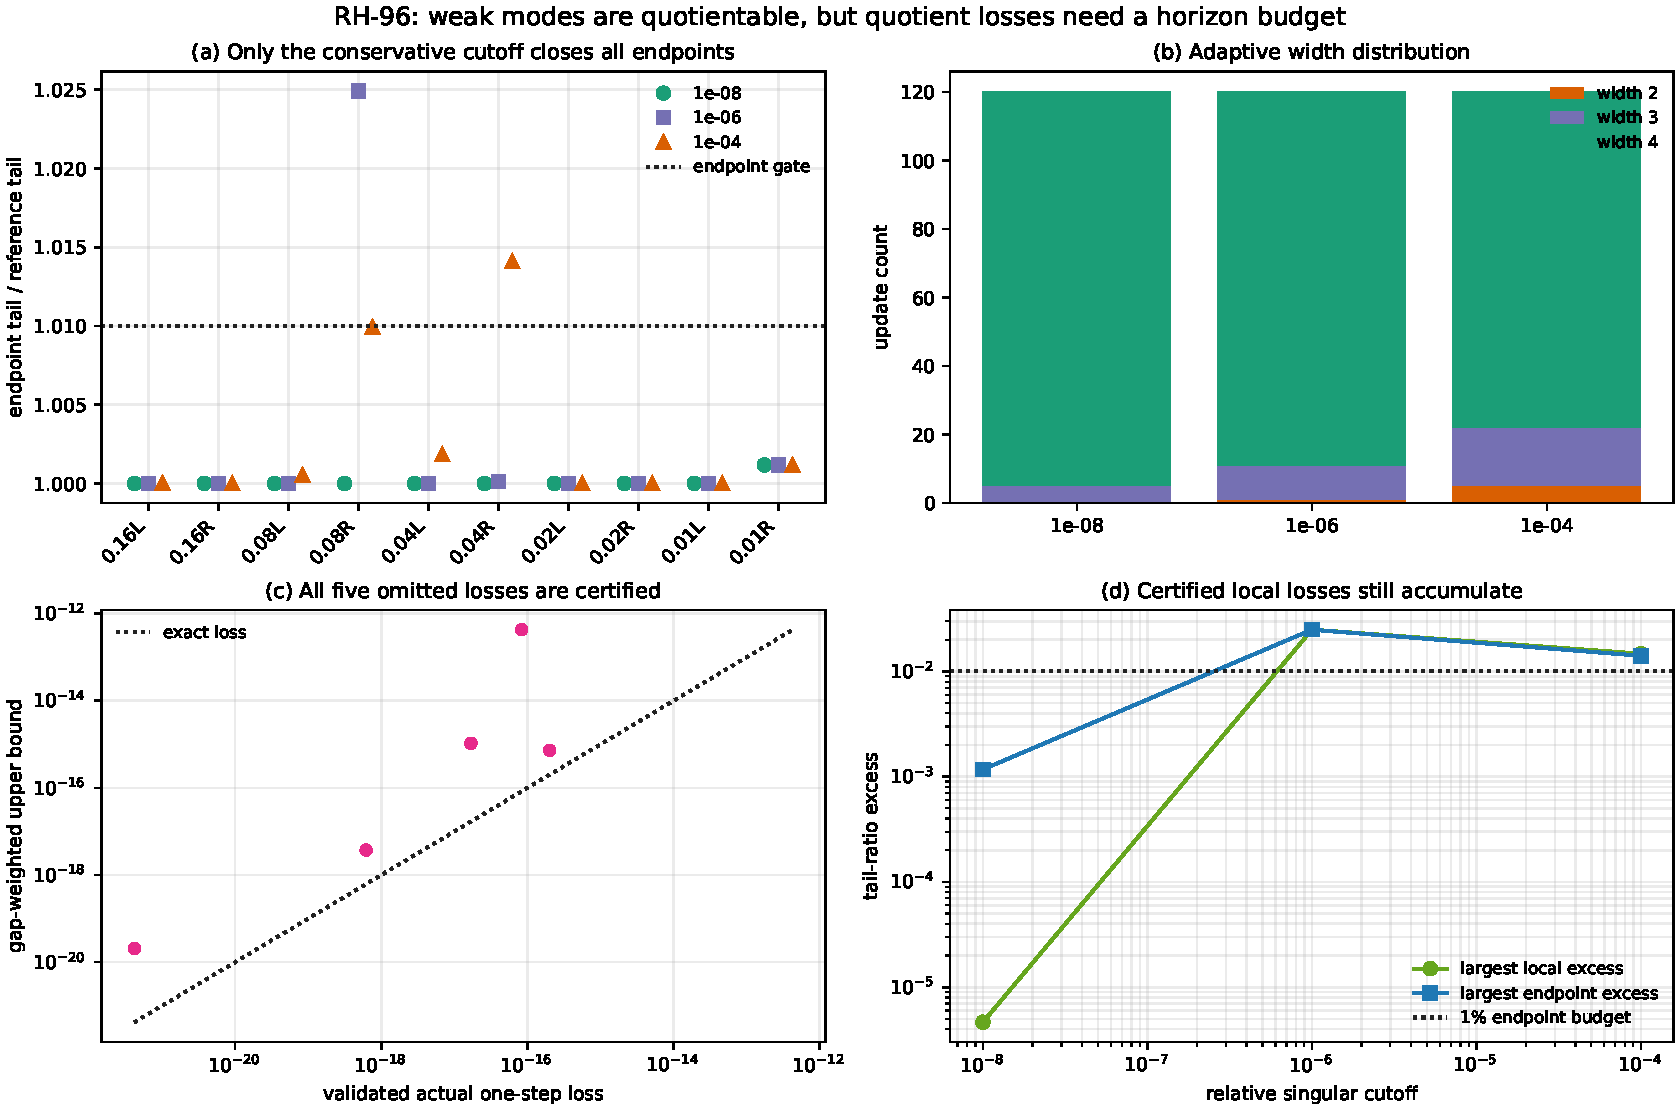
\includegraphics[width=\textwidth]{figures/gap_weighted_weak_mode_quotient.pdf}
\caption{Weak-mode quotient audit.  The $10^{-8}$ cutoff removes exactly five
ill-conditioned modes and preserves every endpoint.  More aggressive local
quotients remain individually certified but fail after recursive
accumulation.}
\label{fig:audit}
\end{figure}

\section{Toward a horizon quotient budget}
\label{sec:horizon}

Let $E_t$ denote the tail excess of an adaptive packet relative to a reference
full-width chain.  The new theorem supplies a local injection
$\varepsilon_t$, but a horizon theorem must also control sensitivity to an
incoming packet error.  The natural recurrence is
\begin{equation}
 E_t\le\rho_tE_{t-1}+\varepsilon_t,
 \label{eq:recurrence}
\end{equation}
where $\rho_t$ measures predictor/refresh amplification.  Iteration yields
\begin{equation}
 E_N\le
 \sum_{j=1}^N\varepsilon_j
 \prod_{\ell=j+1}^N\rho_\ell.
 \label{eq:duhamel}
\end{equation}

The RH-93 block budgets suggest that products of later $\rho_\ell$ may be
contractive even when individual factors exceed the desired target.  A useful
RH-97 result should therefore combine:
\begin{itemize}[leftmargin=2em]
\item the gap-weighted injections from \cref{thm:gap};
\item an a posteriori Lipschitz or projective sensitivity factor for one Ritz
refresh;
\item four-step products rather than rigid pointwise bounds;
\item an endpoint budget stated relative to the ambient reference tail.
\end{itemize}
Such a theorem would explain why five tiny omissions survive but eleven
larger ones do not.

\section{Claim boundary}

The universal omitted-block bound and the gap-weighted weak-mode tail-loss
theorem are exact finite-dimensional statements.  The $10^{-8}$ adaptive
chain is validated only on the ten frozen horizons.  We do not prove:
\begin{enumerate}[leftmargin=2em]
\item a uniform retained-to-omitted gap or a universal relative cutoff;
\item a horizon composition inequality of the form \eqref{eq:recurrence};
\item a uniform adaptive-width or repeated-block contraction law;
\item an ambient-free continuum implementation;
\item Stage-A closure, a Hilbert--Polya operator, zeta-zero identification, or
the Riemann Hypothesis.
\end{enumerate}

\section{Conclusion}

The nearly null fourth projected-cross mode need not be reconstructed.  A
gap between the retained rank-$r$ Ritz cutoff and the omitted diagonal
spectrum converts its coupling into the explicit loss bound
$\norm C_F^2/(\alpha-\beta)$.  At cutoff $10^{-8}$, this quotient removes all
five ill-conditioned modes and preserves every source-to-endpoint gate.

The aggressive-cutoff experiments locate the next wall just as clearly:
local certificates do not compose automatically.  The route now needs a
Duhamel-type horizon budget that transports each certified quotient loss
through subsequent reduced Ritz updates.

\bibliographystyle{plainnat}
\bibliography{references}

\end{document}
